\documentclass[11pt]{article}
\usepackage{amsmath}
\usepackage{graphicx}
%Gummi|065|=)
\title{}
\author{}
\date{}
\begin{document}

\maketitle

\section{ table}

\begin{table}[H]
\centering
\begin{tabular}{|l|l|l|}
\hline
\textbf{Variable} &\textbf{Used as}\\
\hline
Income       &Continuous variable	&Annual Income of Household  \\
Sex          &Factor with 2 levels	&1. Male 2. Female\\
Marital      &Factor with 5 levels	&1. Married 2. Living together, not married 3. Divorced or separated 4. Widowed 5. Single, never married\\
Age          &Continuous variable	&1. 14 thru 17 2. 18 thru 24 3. 25 thru 34 4. 35 thru 44 5. 45 thru 54 6. 55 thru 64 7. 65 and Over\\
Edu          &Factor with 6 levels	&1. Grade 8 or less 2. Grades 9 to 11 3. Graduated high school 4. 1 to 3 years of college 5. College graduate 6. Grad Study\\
Occupation   &Factor with 9 levels	&1. Professional/Managerial 2. Sales Worker 3. Factory Worker/Laborer/Driver 4. Clerical/Service Worker 5. Homemaker 6. Student, HS or College 7. Military 8. Retired 9. Unemployed\\
Lived        &Factor with 5 levels	&HOW LONG HAVE YOU LIVED IN THE SAN FRAN./OAKLAND/SAN JOSE AREA? 1. Less than one year 2. One to three years 3. Four to six years 4. Seven to ten years 5. More than ten years\\
Dual\_Income &Factor with 3 levels	&DUAL INCOMES (IF MARRIED) 1. Not Married 2. Yes 3. No\\
Household    &Continuous variable	&PERSONS IN YOUR HOUSEHOLD 1. One 2. Two 3. Three 4. Four 5. Five 6. Six 7. Seven 8. Eight 9. Nine or more\\
Householdu18 &Continuous variable	&PERSONS IN HOUSEHOLD UNDER 18 0. None 1. One 2. Two 3. Three 4. Four 5. Five 6. Six 7. Seven 8. Eight 9. Nine or more\\
Status       &Factor with 3 levels	&HOUSEHOLDER STATUS 1. Own 2. Rent 3. Live with Parents/Family\\
Home\_Type   &Factor with 5 levels	&1. House 2. Condominium 3. Apartment 4. Mobile Home 5. Other\\
Ethnic       &Factor with 8 levels	&1. American Indian 2. Asian 3. Black 4. East Indian 5. Hispanic 6. Pacific Islander 7. White 8. Other\\
Language     &Factor with 3 levels	&WHAT LANGUAGE IS SPOKEN MOST OFTEN IN YOUR HOME? 1. English 2. Spanish 3. Other\\
\hline
\end{tabular}
\caption{variables}
\label{variables}
\end{table}



\section{ Frequentinst Linear Model }
hgjhg


\section{Linear Model Selection and Regularization}  
The concept of the Linear Model Selection and Regularization is to improve the linear model by replacing the plain least squares fitting with an alternative fitting procedure that might lose a little bit of fitting but yields better predictive performance and model interpretability. 

The relative approaches that follow are the Subset Selection and the Shrinkage. The first, involves identifying a subset of p predictors that we believe to be related to the response and then fitting the model using least squares on the reduced set of variables. The second, involves fitting the model using all p predictors but the coefficients are shrunken towards zero (or exactly zero depending on the method used) relative to the least squares estimates, in order to reduce the variance. From the first category we will use the Best Subset Selection and from the second the Lasso.

\subsection{Best Subset Selection}

In the Best Subset Selection we begin by fitting all p models $\binom{p}{2}$ models that contain exactly one predictor, all $\binom{p}{2} =\frac{p(p-1)}2$ models that contain exactly two predictors and so forth and finally we look at the resulting models and try to identify the best model.

In our example the initial marketing data contain 13 predictors and the response, after the factorizing we get 42 variables and the intercept. After fitting the model using Best Subset Selection for various numbers of variables we observed that the indicators that we examine in this method, the adjusted R, the BIC and the Cp suggested that we use more variables to fit the model. To be more precise the more variables added, the best the indicators turned out to be. So for model simplicity and in order to avoid overfitting, we decided to use the first 13 variables that are considered the most important by the model(the model uses the lowest RSS as criteria). In the text below we can see which predictors are considered to be the most important according to the Best Subset Solution.


\begin{verbatim}
          Sex2 Marital2 Marital3 Marital4 Marital5 Age Edu2 Edu3 Edu4

13  ( 1 ) " "  " "      " "      " "      " "      "*" " "  "*"  "*" 
          Edu5 Edu6 Occupation2 Occupation3 Occupation4 Occupation5
      
13  ( 1 ) "*"  "*"  " "         " "         "*"         " "        
          Occupation6 Occupation7 Occupation8 Occupation9 Lived2 Lived3

13  ( 1 ) "*"         " "         "*"         "*"         " "    " "   
          Lived4 Lived5 Dual_Income2 Dual_Income3 Household Householdu18
      
13  ( 1 ) " "    " "    "*"          "*"          " "       " "         
          Status2 Status3 Home_Type2 Home_Type3 Home_Type4 Home_Type5
   
13  ( 1 ) "*"     "*"     " "        " "        " "        " "       
          Ethnic2 Ethnic3 Ethnic4 Ethnic5 Ethnic6 Ethnic7 Ethnic8
 
13  ( 1 ) " "     " "     " "     " "     " "     " "     " "    
          Language2 Language3
    
13  ( 1 ) " "       " " 
\end{verbatim}

Let Y indicate the response which in our case is the income. Then the model according to the Best Subset Selection will be:

Y= $\beta$0 + $\beta$1Age + $\beta$2Edu3 + $\beta$3Edu4 + $\beta$4Edu5 + $\beta$5Edu6 + $\beta$6Occupation4 + $\beta$7Occupation6 + $\beta$8Occupation8 + $\beta$9Occupation9 + $\beta$10Dual\_Income2+ $\beta$11Dual\_Income3 + $\beta$12Status2 + $\beta$13Status3

We conclude that income is influenced by the Age and the level of education and more precisely by the higher levels of education. Furthermore it is affected by the two most extreme occupation categories, the Clerical/Service Worker and the unemployed as well as the Students and the retired. The dual income is an other factor that affects our response and the status of the householder as well and more specifically the factors related to the fact that the householder might be paying a rent or living with his parents/family. 

Below we can also see how the $R^2$ is formulated while adding more variables.

\begin{verbatim}
[1] 0.1754538 0.2667926 0.3102752 0.3386352 0.3570837 0.3771129 0.3958195 0.4064571
[9] 0.4164211 0.4221043 0.4276303 0.4322475 0.4365138
 \end{verbatim}
 
and we see that the $R^2$ statistics increases from 17,55\% when only 1 variable is included in the model to 43,65\% when we use 13 variables, which means that  the model explains 43,65\% of the variability of the response data around its mean when we use these 13 predictors.

The next step is to see the plots produced for RSS, adjusted $R^2$ , Cp and BIC
\begin{figure}[h]
    \centering
   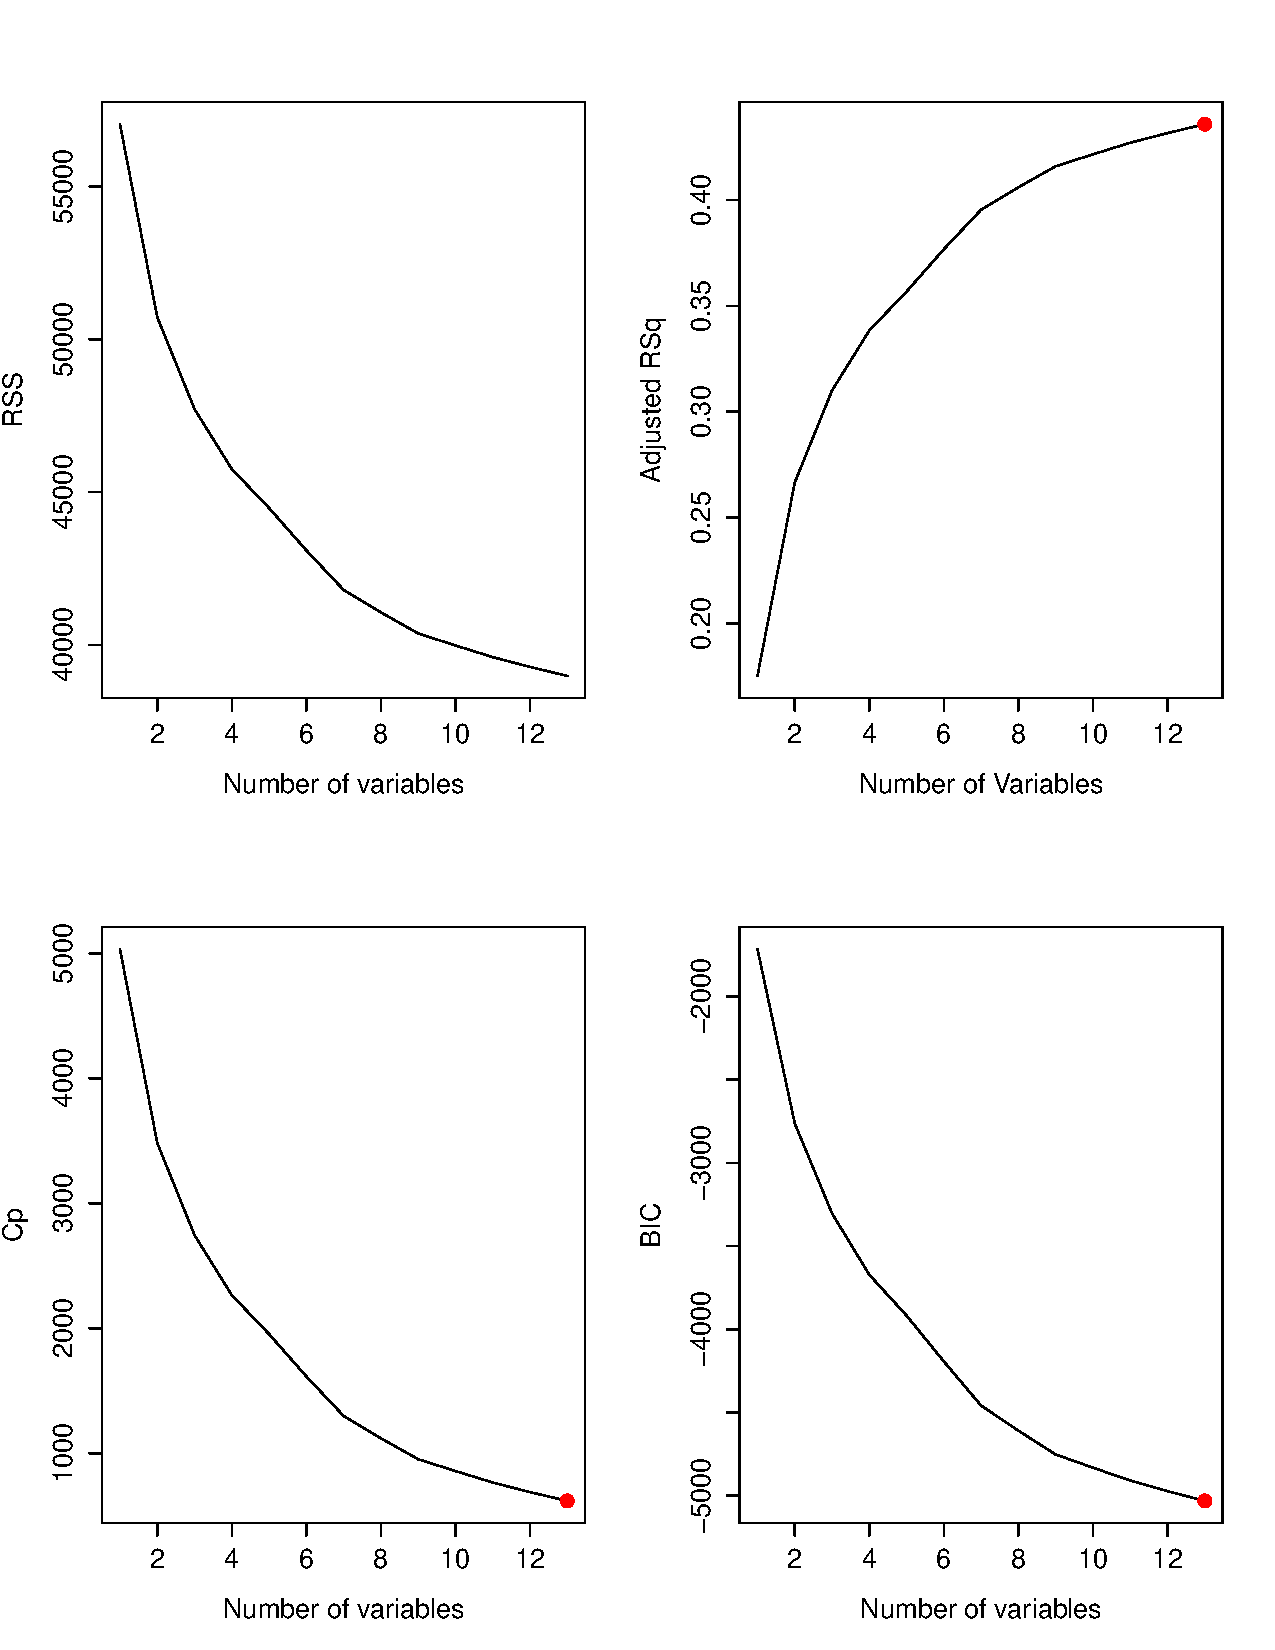
\includegraphics[scale=0.3]{RSS_ETC_PLOT.pdf}
    \caption{Plots of RSS, adjusted $R^2$, Cp and BIC} 
    \label{fig:Plots of RSS, adjusted $R^2$, Cp and BIC}
\end{figure} 


If we use BIC as the selection criteria, it is suggested that we use a subset of thirteen predictors(as expected) that are believed to be related to the response as BIC reaches its lowest value when it uses thirteen predictors. To see which thirteen predictors we plot the BIC and get the following figure that results to the model mentioned previously.
\DeclareGraphicsExtensions{.pdf,.png,.jpg}
\begin{figure}[h]
    \centering
   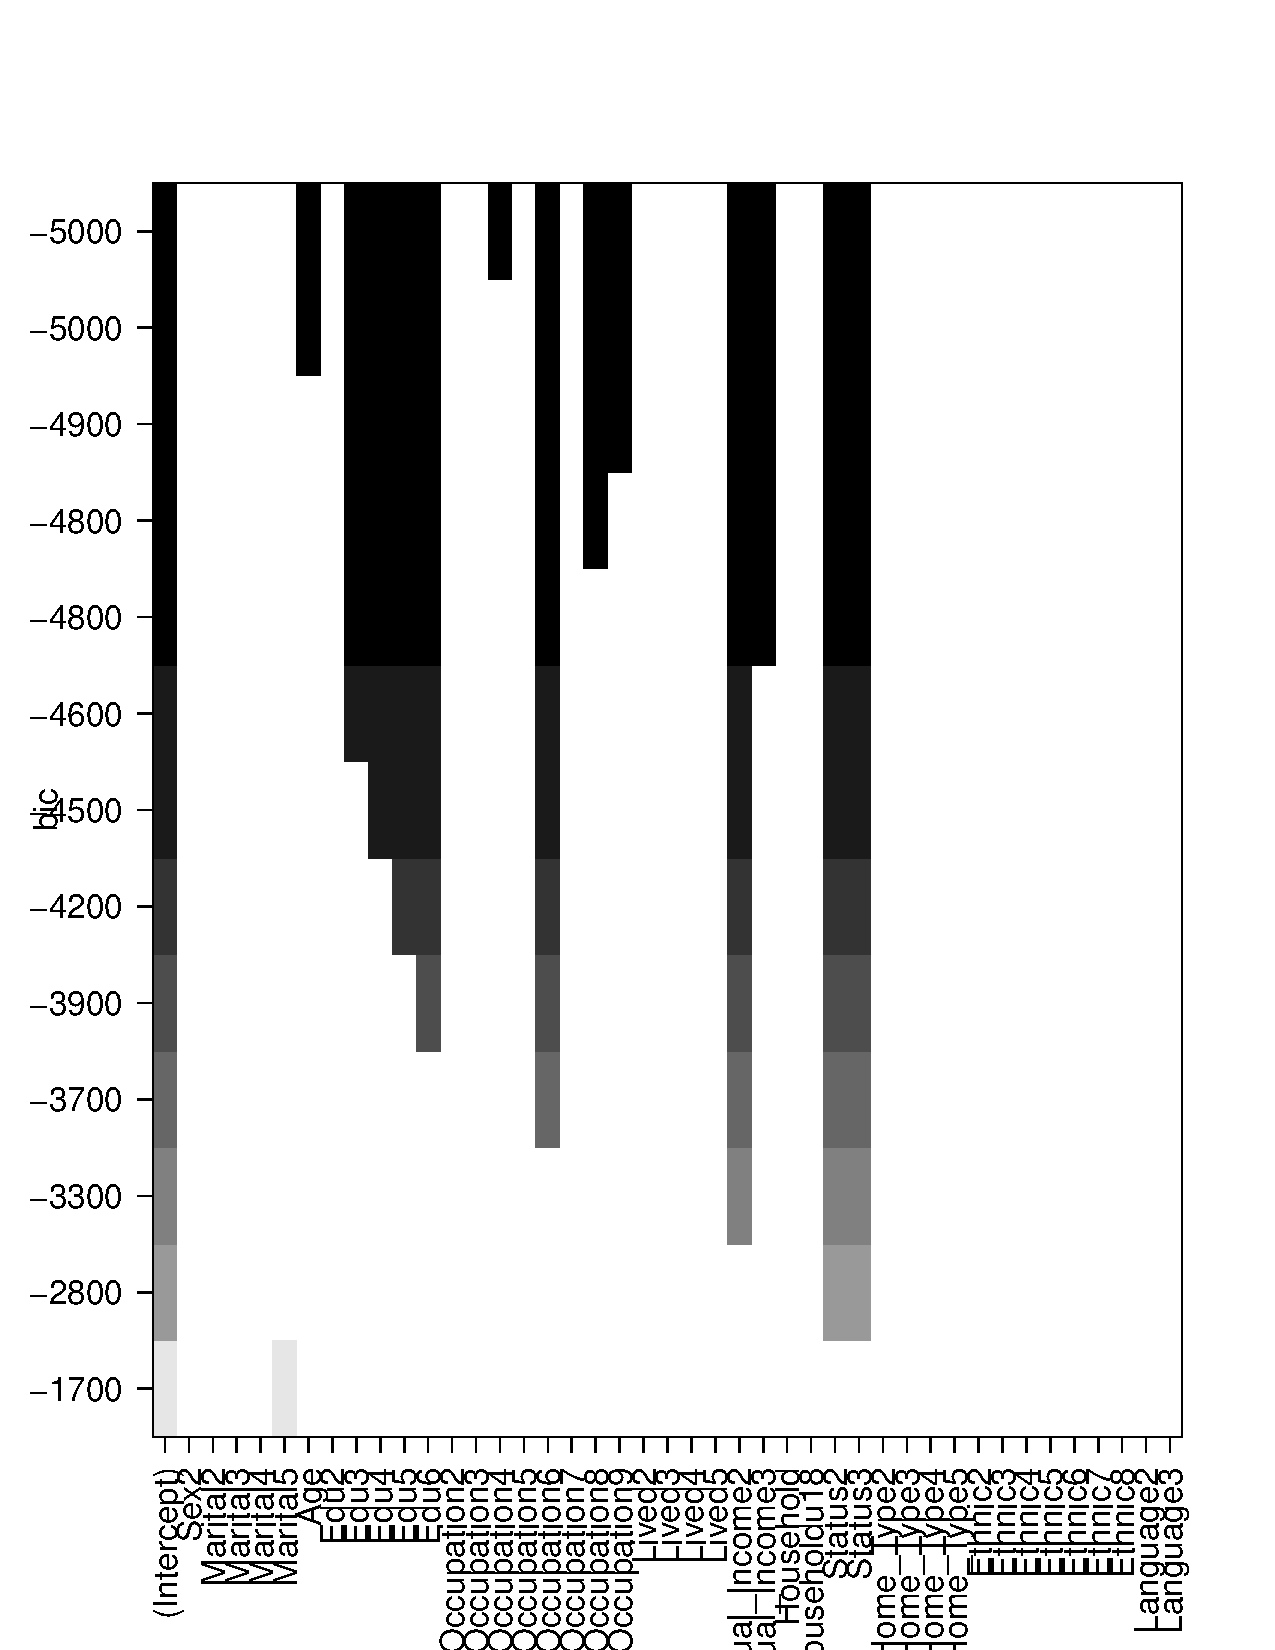
\includegraphics[scale=0.3]{BIC_PLOT.pdf}
    \caption{Selected variables for the best model ranked according to BIC}
    \label{fig:Selected variables for the best model ranked according to BIC}
\end{figure}


The disadvantage of the above indicators (including BIC) is that they all adjust the training error, so in the next part we are going to use the cross validation that estimates the test error directly.

\subsection{Cross Validation}
We are interested in the test error which is the average error that results from using a statistical learning method to predict a response on a new observation, which means a measurement that was not used in training the method. 

So we use the cross validation which is a method that estimates the test error holding out a subset  of the training observations from the fitting process and then applying the statistical learning method to those held out observations. Again for model simplicity we choose to use up to 13 variables to the resulting model because the more variables we added the lowest the test MSE was getting.

\begin{figure}[h]
    \centering
   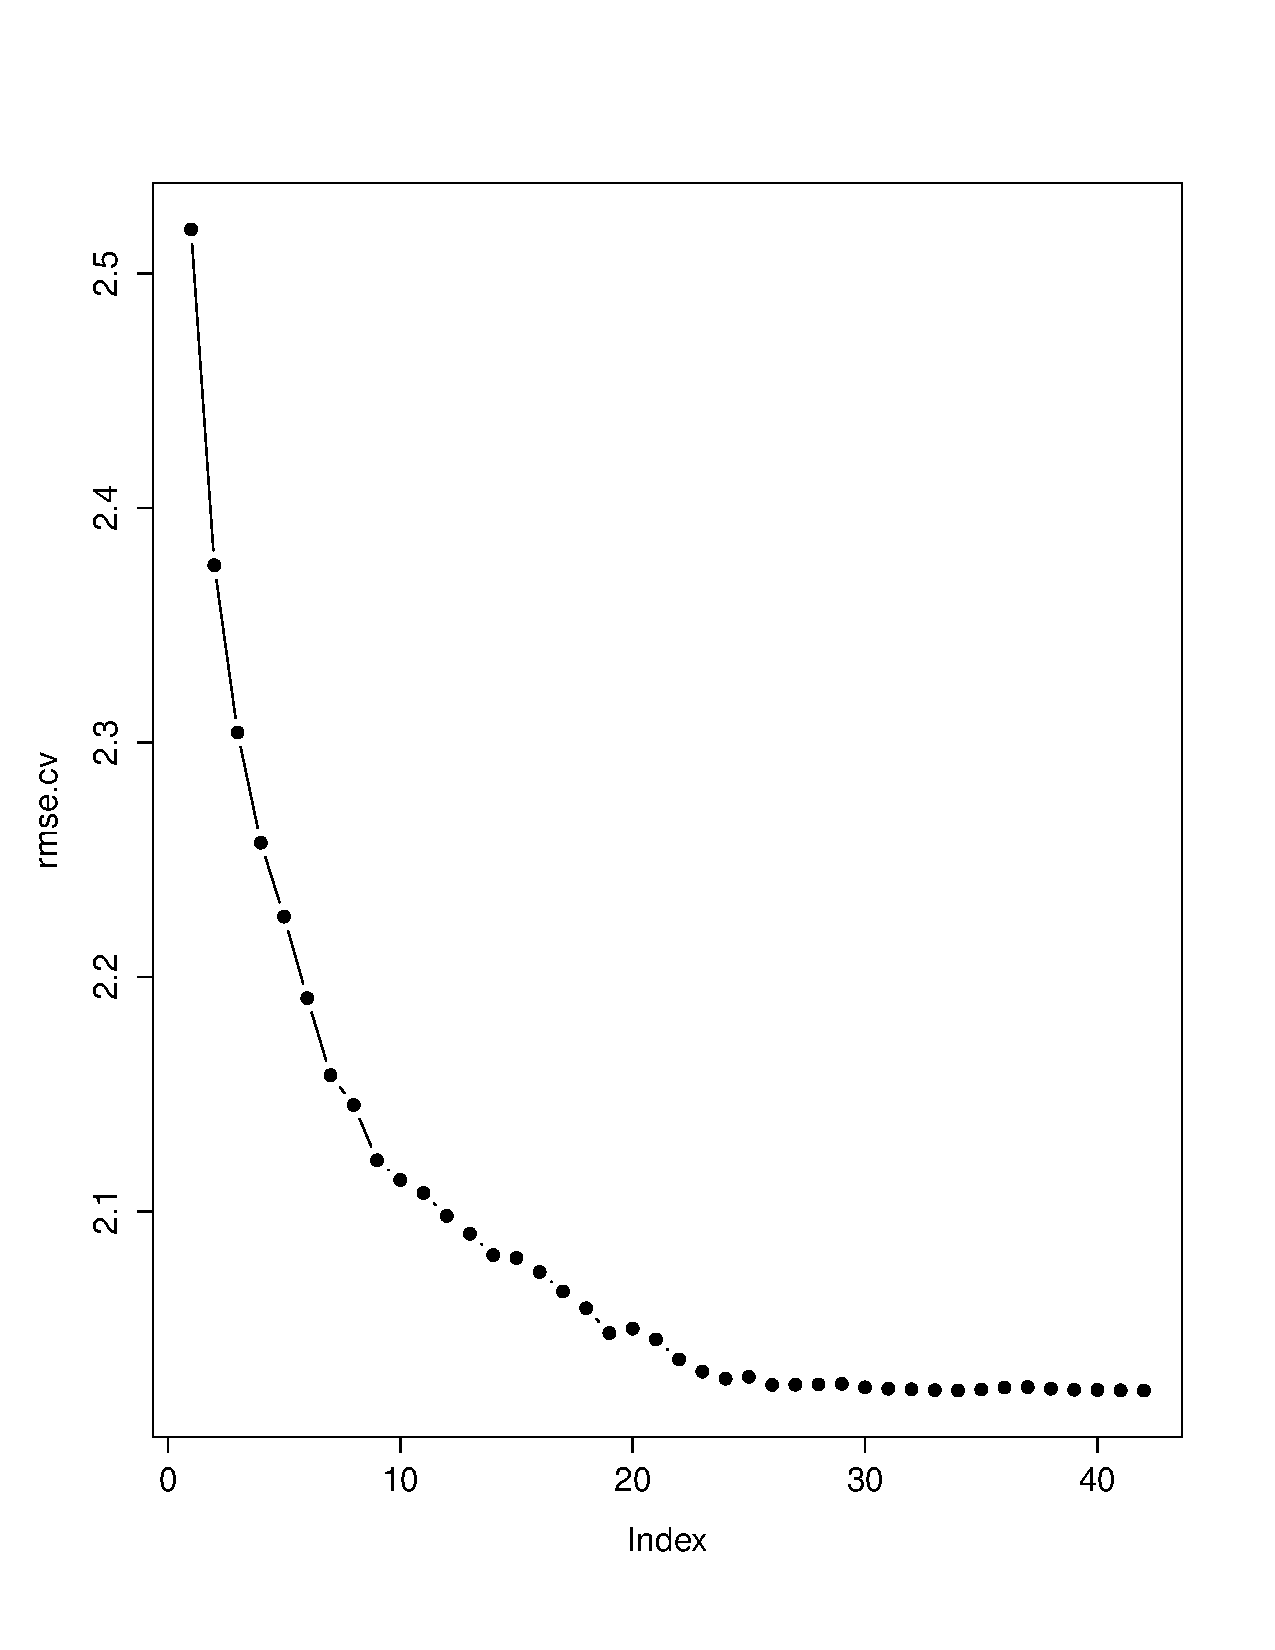
\includegraphics[scale=0.3]{CROSS_VALIDATION_MSE_PLOT.pdf}
    \caption{Cross validation Error}
    \label{fig:Cross validation Error}
\end{figure}

From which we can see that cross-validation selects a 13 variable model with coefficients:
\begin{verbatim}
 (Intercept)          Age         Edu3         Edu4         Edu5 
   3.5684152    0.2091928    0.9963787    1.5503228    2.2064117 
        Edu6  Occupation4  Occupation6  Occupation8  Occupation9 
   2.5584260   -0.5856842   -1.2213397   -1.5116519   -1.1271196 
Dual_Income2 Dual_Income3      Status2      Status3 
   1.3589114    0.8069902   -1.4836791   -0.8627755 
 \end{verbatim}
The above coefficients constitute the coefficients of the model mentioned in the previous section.

\subsection{The lasso}
Unlike Best Subset Selection presented in a previous subsection the Lasso includes all p predictors and uses a penalty depending on the tuning parameter $\lambda$ to perform a variable selection by shrinking the coefficients to zero if $\lambda$ is sufficiently large.

In the Lasso the best $\lambda$ is selected according to the variable which presents the lowest error, but we selected a $\lambda$ = 0.3 as we did not want to have more than approximately 11 variables and the intercept to avoid overfitting. As it expected the more variables added, the less the test error but in our example the higher value of lambda selected did not affect the corresponding test in an important way.

\DeclareGraphicsExtensions{.pdf,.png,.jpg}

\begin{figure}[h]
    \centering
   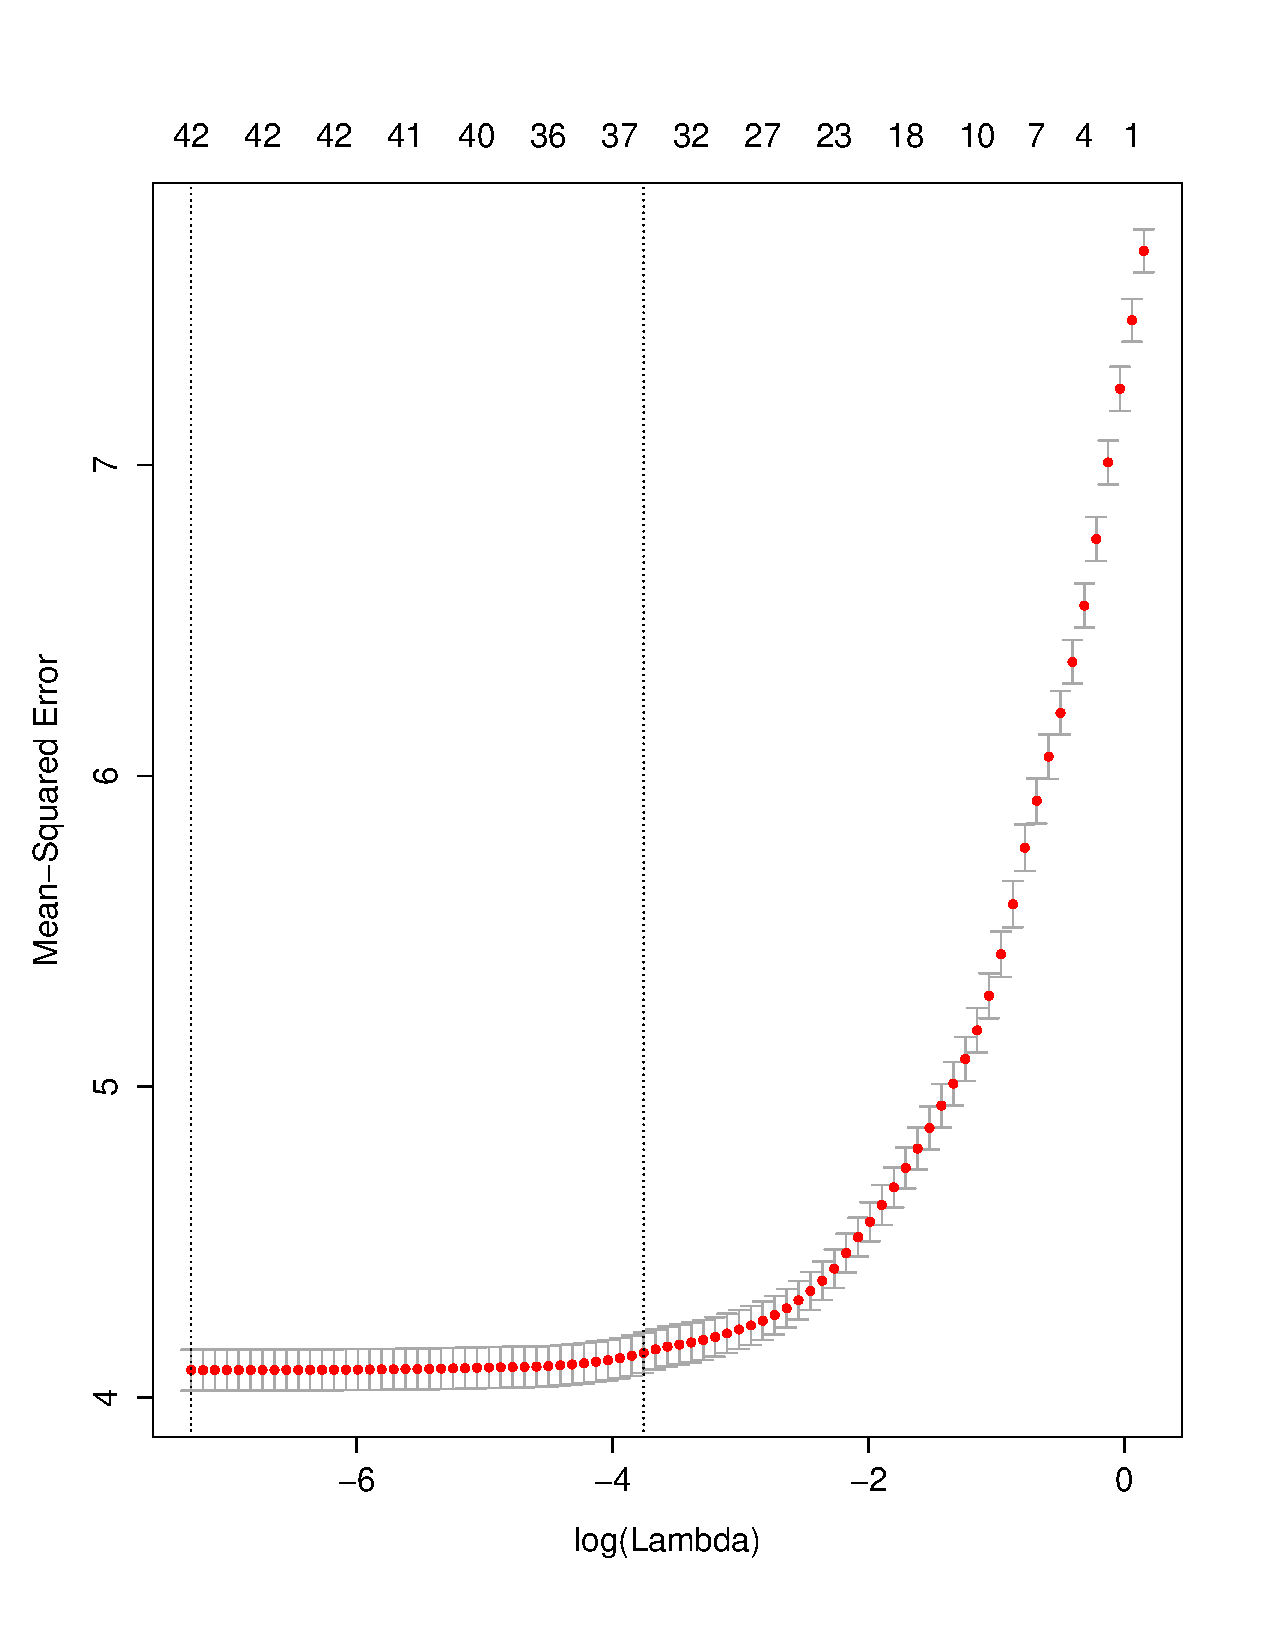
\includegraphics[scale=0.3]{LASSO_ERROR_PLOT.pdf}
    \caption{Plot of the MSE of the Lasso}
    \label{fig:Plot of the MSE of the Lasso}
\end{figure}

Lasso Coefficients
\begin{verbatim}
(Intercept)   4.93382364      
Marital5     -0.49340288
Age           0.11818877
Edu2         -0.58760282      
Edu5          0.33818740
Edu6          0.65078190       
Occupation6  -0.82120634    
Dual_Income2  0.83935922     
Status2      -0.47429447
Status3      -0.49832197       
Home_Type3   -0.21073592      
Ethnic5      -0.02600054
 \end{verbatim} 
 
 The model to which we conclude using the Lasso is slightly different from the one that we got from the Best Subset Selection. Now the 11 variables suggested to be used to fit the model are: the marital status and especially the fact that someone is single as opposed to all the other factors of this variable, the age, the fact that someone is either a college or a university graduate or at Grades 9 to 11. Besides the existence of a dual income and the facts that someone might pay a rent or live with his family affect the Income as well. Some other factors that appear in this model is the home type and the ethnicity that are negatively correlated with our response which means that if someone stays in an apartment or has a hispanic ehtnicity it is more probable that his income is less as opposed to the other factors of the corresponding variables.
\end{document}
